\section{Абстрактные классы и методы}

\begin{frame}[fragile]
	\frametitle{Абстрактные методы}

	Иногда нет смысла в реализации метода, например:
	\begin{minted}[bgcolor=bgcode]{java}
	class Function {
	    float calc(float x) { return 0; }
	}

	class Line extends Function {
	    float k, b;

	    float calc(float x) {
	        return k * x + f;
	    }
	}
	\end{minted}
	В этом случае метод можно описать как abstract:
	\begin{minted}[bgcolor=bgcode]{java}
	abstract float calc(float x);
	\end{minted}
	Это означает что у метода нет реализации.

\end{frame}


\begin{frame}[fragile]
	\frametitle{Абстрактные классы}
	\begin{large}
	Класс в котором есть хотя бы один абстрактный метод --- абстрактный и должен быть описан с ключевым словом \emph{abstract}:

	\begin{minted}[bgcolor=bgcode,linenos=true]{java}
	abstract class Function {
	    abstract float calc(float x);
	};
	\end{minted}

	Мы не можем создавать объекты абстрактных классов, но можем описывать ссылки таких типов, например:
	\begin{minted}[bgcolor=bgcode,linenos=true]{java}
	Function f;
	f = new Function(); /* error */
	f = new Line(10, 15); /* OK */
	\end{minted}
	\end{large}
\end{frame}

\begin{frame}[fragile]
	\frametitle{Часть методов может быть реализована}

	\begin{minted}[bgcolor=bgcode,linenos=true]{java}
	abstract class Function {
	    abstract float calc(float x);

	    void printTable(float a, float b, int n) {
	        for (float x = a; x <= b; x += (b - a) / n)
	             System.out.println(
	                  String.format("%f %f", x, calc(x)));
	    }
	};
	\end{minted}

	В этом случае метод \emph{printTable} будет вызывать \emph{calc}, реализованный в дочернем классе.
\end{frame}

\begin{frame}[fragile]
	\frametitle{Абстрактные классы можно наследовать}
	\begin{minted}[bgcolor=bgcode,linenos=true]{java}
	abstract class A {
	    abstract int method1();
	};

	abstract class B extends A {
	    abstract int method2();
	};

	abstract class C extends B {
	    int method1() { return 10; }
	};

	class D extends C {
	    int method2() { return 20; }
	};
	\end{minted}

	Неабстрактым класс можно объявить только тогда, когда будут реализованы все его методы.
\end{frame}

\section{Интерфейсы}
\begin{frame}[fragile]
	\frametitle{Допустим в Java было бы разрешено множественное наследование}

	\begin{columns}[c]
	\column{2.55in}
	\begin{minted}[bgcolor=bgcode,linenos=true]{java}
	abstract class A {
	    abstract void method1();
	};
	class B extends A {
	    void method1() { return 1; }
	};
	class C extends A {
	    void method1() { return 2; }
	};
	class D extends B, C {
	    void test() {
	        println(method1());
	    }
	};
	\end{minted}
	\column{1.90in}
	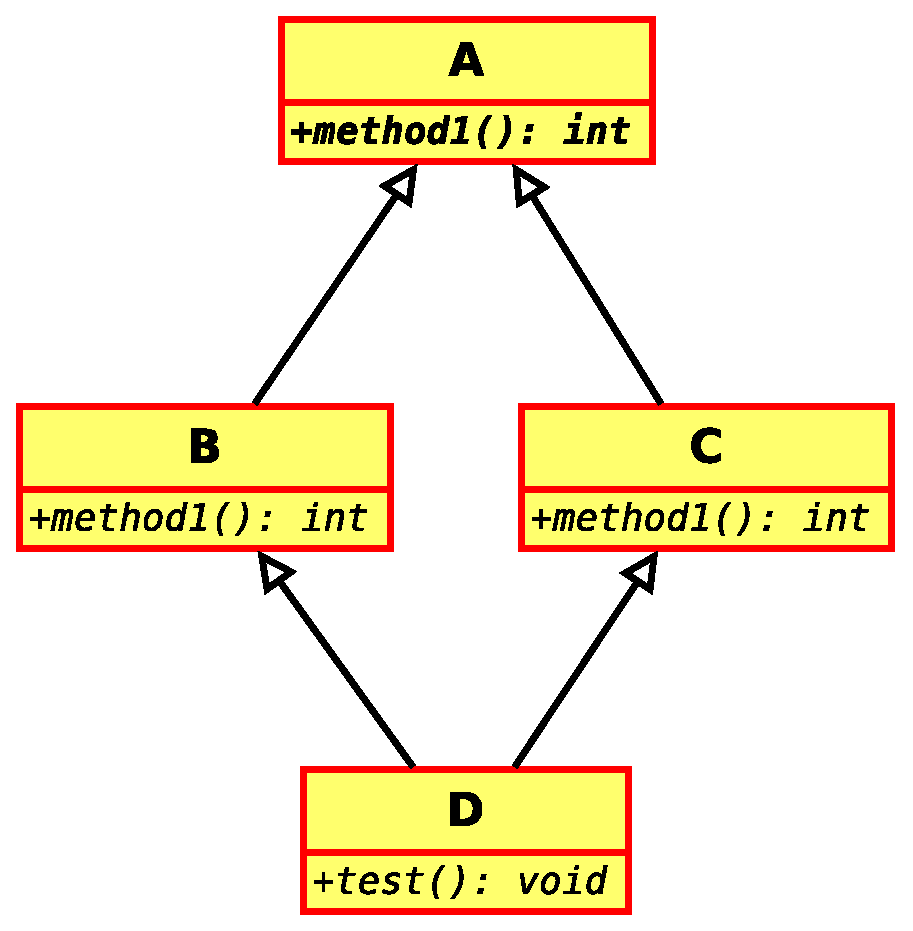
\includegraphics[width=1.9in]{lesson-7-Diagram1.eps}

	\smallskip
	Из какого класса будет вызван \emph{method1()} ?
	\end{columns}
\end{frame}

\begin{frame}[fragile]
	\frametitle{Проблемы с множественным наследованием}
	\begin{large}
	\begin{itemize}
	\item{Ромбовидное наследование, рассмотренное на предыдущем слайде}
	\item{Порядок наследования меняет поведение класса}
	\end{itemize}

	Множественное наследование в чистом виде --- это ошибка проектирования.
	\end{large}
\end{frame}


\begin{frame}[fragile]
	\frametitle{Интерфейсы}
	Интерфейс --- это полностью абстрактный класс, не содержащий никаких полей.

	\medskip
	Описывается с помощью ключевого слова \emph{interface}. Так как все методы и так обязательно должны быть абстрактными, то слово \emph{abstract} писать не нужно.

	\medskip
	В случае интерфейсов вместо термина "наследует" используют термин "реализует", вместо ключевого слова \emph{extends} используется \emph{implements}.

	\begin{minted}[bgcolor=bgcode]{java}
	interface X {
	    int method1();
	};

	class A implements X {
	    int method1() { return 10 };
	};
	\end{minted}
\end{frame}

\begin{frame}[fragile]
	\frametitle{Пример}

	\begin{minted}[bgcolor=bgcode,linenos=true]{java}
	interface Clickable {
	    void press();
	    void release();
	};
	interface Drawable {
	    void draw(Graphics g);
	};
	class Button implements Clickable, Drawable {
	    int state = 0;

	    void press { state  = 1; };
	    void release { state = 0; };
	    void draw(Graphics g) {
	        g.drawRect(0, 0, 20, 10);
	        g.drawString("OK", 5, 5);
	    }
	};
	\end{minted}

\end{frame}

\begin{frame}[fragile]
	\frametitle{Использование ссылок на интерфейс}

	Ссылки на интерфейс используются так же как и ссылки на абстрактные классы --- мы можем их описать, присвоить им ссылку на объект, который реализует данный интерфейс, но экземпляр интерфейса создать нельзя.

	\begin{minted}[bgcolor=bgcode,linenos=true]{java}
	Button b = new Button();
	Clickable c = b;
	Drawable d = b;

	b.press();
	c.release();

	d.draw(g);
	\end{minted}
\end{frame}

\begin{frame}[fragile]
	\frametitle{Задача}

	Сделать абстрактный класс \emph{Function} с абстрактным методом для вычисления значения функции и реализованным --- для рисования графика.
	\begin{minted}[bgcolor=bgcode]{java}
	abstract class Function {
	    abstract float calc(float x);
	    void draw(Graphics g) {
	        ...
	    }
	}
	\end{minted}

	Унаследовать от Function классы \emph{Line} и \emph{Parabola}, в которых метод для вычисления значения функции реализован.
	Проверить работу классов с помощью явно заданных в методе main значений.

	Пример рисования с записью в графический файл --- \href{http://lk4.mipt.ru/153/examples/DrawToFile.java}{http://lk4.mipt.ru/153/examples/DrawToFile.java}.
\end{frame}
